\section{Project Description}
\label{section:description}

The main contribution of this work should be to evaluate the boundaries of conventional machine learning approaches for hate speech detection. This includes manual feature extraction and subsequent text classification of doc\-u\-ments into hate speech and non-hate speech as opposed to modern deep learning approaches. Part of this work is also to find out which features and classifiers are suitable for such a classification task. The results should show which features work best for which classifier as well as which problems can be addressed with conventional machine learning methods and which not. A comparison to modern deep learning approaches should be drawn using the metrics of simple accuracy as well as precision and recall, respectively the F1-score. 

As stated above, the two data sets from \cite{ThomasDavidson.2020} and \cite{OnadeGibert.2020} will be used for this project. One possible problem could be that the amount of documents classified as pure hate speech in \cite{ThomasDavidson.2020} might not be enough to create profound classifiers. In this case one has to evaluate whether hate speech data from \cite{OnadeGibert.2020} is enough to achieve valid results or whether documents classified as offensive language from \cite{ThomasDavidson.2020} should be used as hate speech data as well. 

\vspace{12pt}
To summarize the scope of the project the following subgoals were iden\-ti\-fied:

\begin{itemize}
	\item Prepare the data sets.
	\item Identify suitable feature representations and transform the data ac\-cord\-ingly.
	\item Identify and train machine learning classifiers.
	\item Combine classifiers with different feature representations.
	\item Evalute and compare the performance using accuracy, precision, recall and F1-score.
	\item Show the boundaries of conventional machine learning approaches in comparison to deep learning approaches.
\end{itemize}

\begin{figure}[]
	\centering
	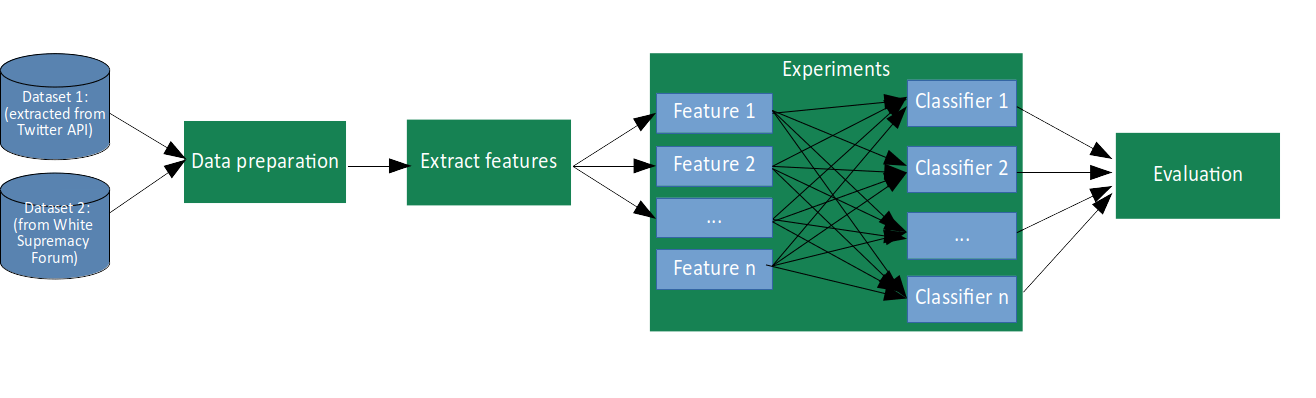
\includegraphics[width=1.0\textwidth]{./pipeline.png}	
	\caption{Text Analytics Pipeline [own representation]}
	\label{fig:pipeline}
\end{figure}

The results of the project can contribute to offer an easier way to detect hate speech without having to train deep neural networks. It furthermore gives a more holistic view on different approaches to handle hate speech detection with conventional machine learning and text analytics methods.

\noindent
[Pipeline Figure]

%TODO: Advantages and disadvantages of specific evaluation methods
%TODO: Identify baseline scores
